\documentclass[../TDE8_filtrage.tex]{subfiles}%

\begin{document}
\section[s]"1"{Filtre avec une bobine}
On considère le circuit ci-contre, avec $R = \SI{1.0}{k\Omega}$ et $L =
	\SI{10}{mH}$, donnant le diagramme de \textsc{Bode} ci-dessous~:
\smallbreak
\noindent
\begin{minipage}[c]{.49\linewidth}
	~
	\begin{center}
		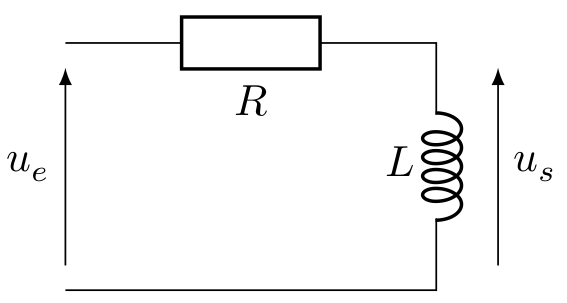
\includegraphics[width=\linewidth]{filtrebob_plain}
	\end{center}
\end{minipage}
\hfill
\begin{minipage}[c]{.49\linewidth}
	~
	\begin{center}
		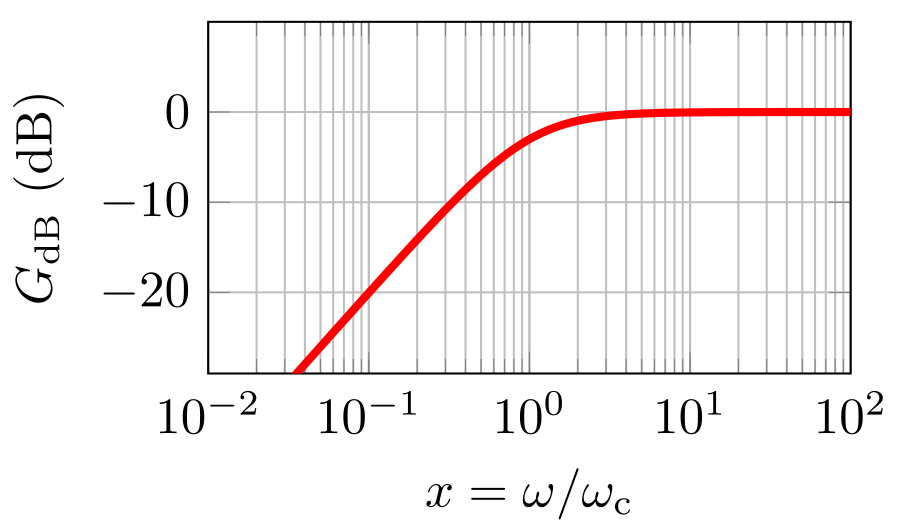
\includegraphics[width=\linewidth]{filtrebob_bode}
	\end{center}
\end{minipage}

\QR{%
	Sans utiliser le diagramme de \textsc{Bode}, quelle est la nature
	du filtre~?
}{%
	À basses fréquences, $\abs{\Zu_L} \opto{}{\w\ra0} 0$, donc
	$H(\w) \opto{}{\w\ra0} 0$. À hautes fréquences,
	$\abs{\Zu_L} \opto{}{\w\ra\infty} \infty$, donc
	$H(\w) \opto{}{\w\ra\infty} 1$~: \textbf{c'est un
		passe-haut}.
}

\QR{%
	Déterminer sa fonction de transfert et l'écrire sous la forme
	\[\Hu(\jw) = H_0 \frac{\jj\dfrac{\w}{\w_c}}{1 +
			\jj\dfrac{\w}{\w_c}}\]
	avec $H_0$ et $\w_c$ des constantes à préciser.
}{%
	On fait un pont diviseur de tension~:
	\begin{gather*}
		\xul{u_s} = \frac{\jlw}{R + \jlw}\xul{u_e}
		\Lra
		\frac{\xul{u_s}}{\xul{u_e}} = \Hu =
		\cancel{\frac{R}{R}}\times\frac{\jj\w\frac{L}{R}}{1 + \jj\w
			\frac{L}{R}}\\
		\Lra
		\boxed{\Hu(\jj\w) = H_0 \frac{\jj\frac{\w}{\w_c}}{1 +
				\jj\frac{\w}{\w_c}}}
		\qavec
		\boxed{H_0 = 1
			\qet
			\w_c = \frac{R}{L} = \SI{1e5}{rad.s^{-1}}}
	\end{gather*}
}

\QR{%
	Montrer par le calcul que la pente de l'asymptote du diagramme
	de \textsc{Bode} pour $\w \ll \w_c$ est de \SI{20}{dB/décade}.
}{%
	$1 + \jj \frac{\w}{\w_c} \underset{\w \ll \w_c}{\sim} 1$, et donc
	\begin{gather*}
		\Hu(\jj\w) \underset{\w\ll\w_c}{\sim} \jj \frac{\w}{\w_c}
		\Lra
		\boxed{G_{\rm dB} = 20\log \left( \abs{\Hu} \right)
			\underset{\w\ll\w_c}{\sim} 20\log x}
	\end{gather*}
	d'où la pente de \SI{20}{dB/décade}.
}

\QR{%
	On considère une tension d'entrée $u_e(t)$ somme de 3 harmoniques de
	mêmes amplitudes, de mêmes phases initiales, mais de fréquences
	respectives $f_1 = \SI{100}{Hz}$, $f_2 = \SI{1}{kHz}$ et $f_3 =
		\SI{100}{kHz}$. Donner le spectre de sortie.
}{%
	On trouve le spectre de sortie en multipliant chaque amplitude
	d'entrée par le module de la fonction de transfert pour avoir
	l'amplitude de sortie. \textbf{Attention, pulsation $\neq$ fréquence}.
	On a
	\[\abs{\Hu(f)} = \frac{\dfrac{2\pi f}{\w_c}}{\sqrt{1 +
				\left( \dfrac{2\pi f}{\w_c} \right)^2}}\]
	\begin{itemize}
		\item $H(f_1) \approx \num{6.3e-3}$~: le fondamental est
		      complètement atténué, il ne reste que \num{0.6}\% de son
		      amplitude initiale~;
		\item $H(f_2) \approx \num{6.3e-2}$~: l'harmonique $f_2$ est
		      fortement atténué, il n'en reste que 6\%~;
		\item $H(f_3) \approx \num{0.99}$~: l'harmonique $f_3$ est
		      pratiquement entièrement conservé.
	\end{itemize}
}

\end{document}
